\documentclass[tikz,border=2mm]{standalone}
\usepackage{amssymb}
\usetikzlibrary{patterns,shapes.geometric,calc}

\begin{document}
	
	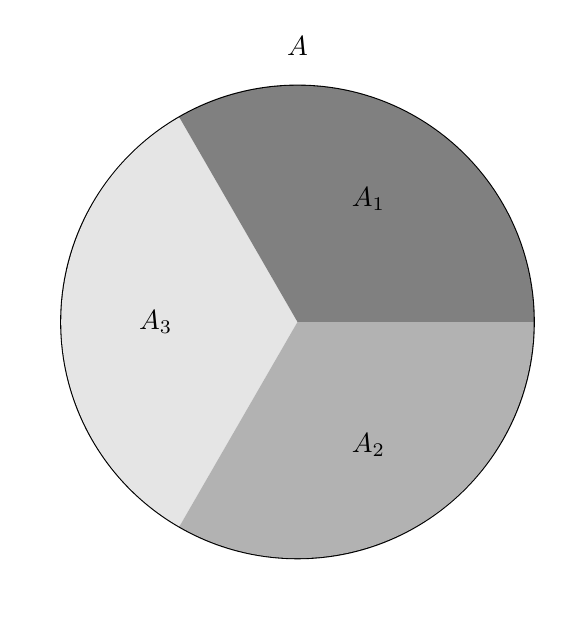
\begin{tikzpicture}
		
		% Draw the set S as a circle
		\draw[thick] (0,0) circle (3);
		\node at (0,3.5) {$A$};
		
		% Draw partitions A, B, and C
		\fill[black!10] (0,0) -- (120:3) arc (120:240:3) -- cycle;
		\fill[black!30] (0,0) -- (240:3) arc (240:360:3) -- cycle;
		\fill[black!50] (0,0) -- (0:3) arc (0:120:3) -- cycle;
		
		% Labels for partitions A, B, and C
		\node at (60:1.8) {$A_1$};
		\node at (300:1.8) {$A_2$};
		\node at (180:1.8) {$A_3$};
		
		
	\end{tikzpicture}
	
\end{document}
